\chapter{Software architecture}
\label{chap:architecture}

\myepigraph{If you think good architecture is expensive, try bad architecture.}{Brian Foote and Joseph Yoder}{Big Ball of Mud}


\section{Multi-process Architecture}

A misbehaving web page could take down the entire system of a web browser. One plug-in bug can bring down an entire browser and all of the currently running tabs. To prevent this, modern operating systems are developed under sandboxed security mechanism. They isolate applications into separate processes that are walled off from one another, this way, a crash in one application generally does not impair other applications or the integrity of the operating system, and each user's access to other users' data is restricted \cite{man}.

Web content has evolved to contain significant amounts of active code that run within the browser, making many web sites more like applications than documents. This evolution has changed the role of the browser into an operating system rather than a simple document renderer. Chromium is built like an operating system to run these applications in a safe and robust way, using multiple OS processes to isolate web sites from each other and from the browser itself. This improves robustness because each process runs in its own address space, is scheduled by the operating system, and can fail independently. In some ways, this brings to web browsing the benefits that memory protection and access control brought to operating systems.

\textit{Grosso modo}, Chromium uses separate processes for browser tabs to protect the overall application from bugs and glitches in the rendering engine. It also serves a purpose in restricting access from each rendering engine process to others and to the rest of the system. We refer to the main process that runs the UI and manages tab and plugin processes as the ``browser process". Likewise, the tab-specific processes are called ``render processes" or ``renderers". The renderers use the Blink open-source layout engine for interpreting and laying out HTML. In contrast, a single-process browser will have all tabs' data randomly distributed in its memory, and it is impossible to separate the used and unused data so cleanly, wasting both memory and performance. Although, there is more than just dividing the processes in case one render crashes. Multi-process architecture makes sure the rendered can not do anything to make the browser hang. Also, the main process driving the user interface can always show a recent representation of the webpage as well as favoring asynchronous and not blocking communication above all else.

Each render process has a global \texttt{RenderProcess} object that manages communication with the parent browser process and maintains global state. The browser maintains a corresponding \texttt{RenderProcessHost} for each render process, which manages browser state and communication for the renderer. The browser and the renderers communicate using Chromium's IPC system. 

\begin{sidewaysfigure}
    \centering
    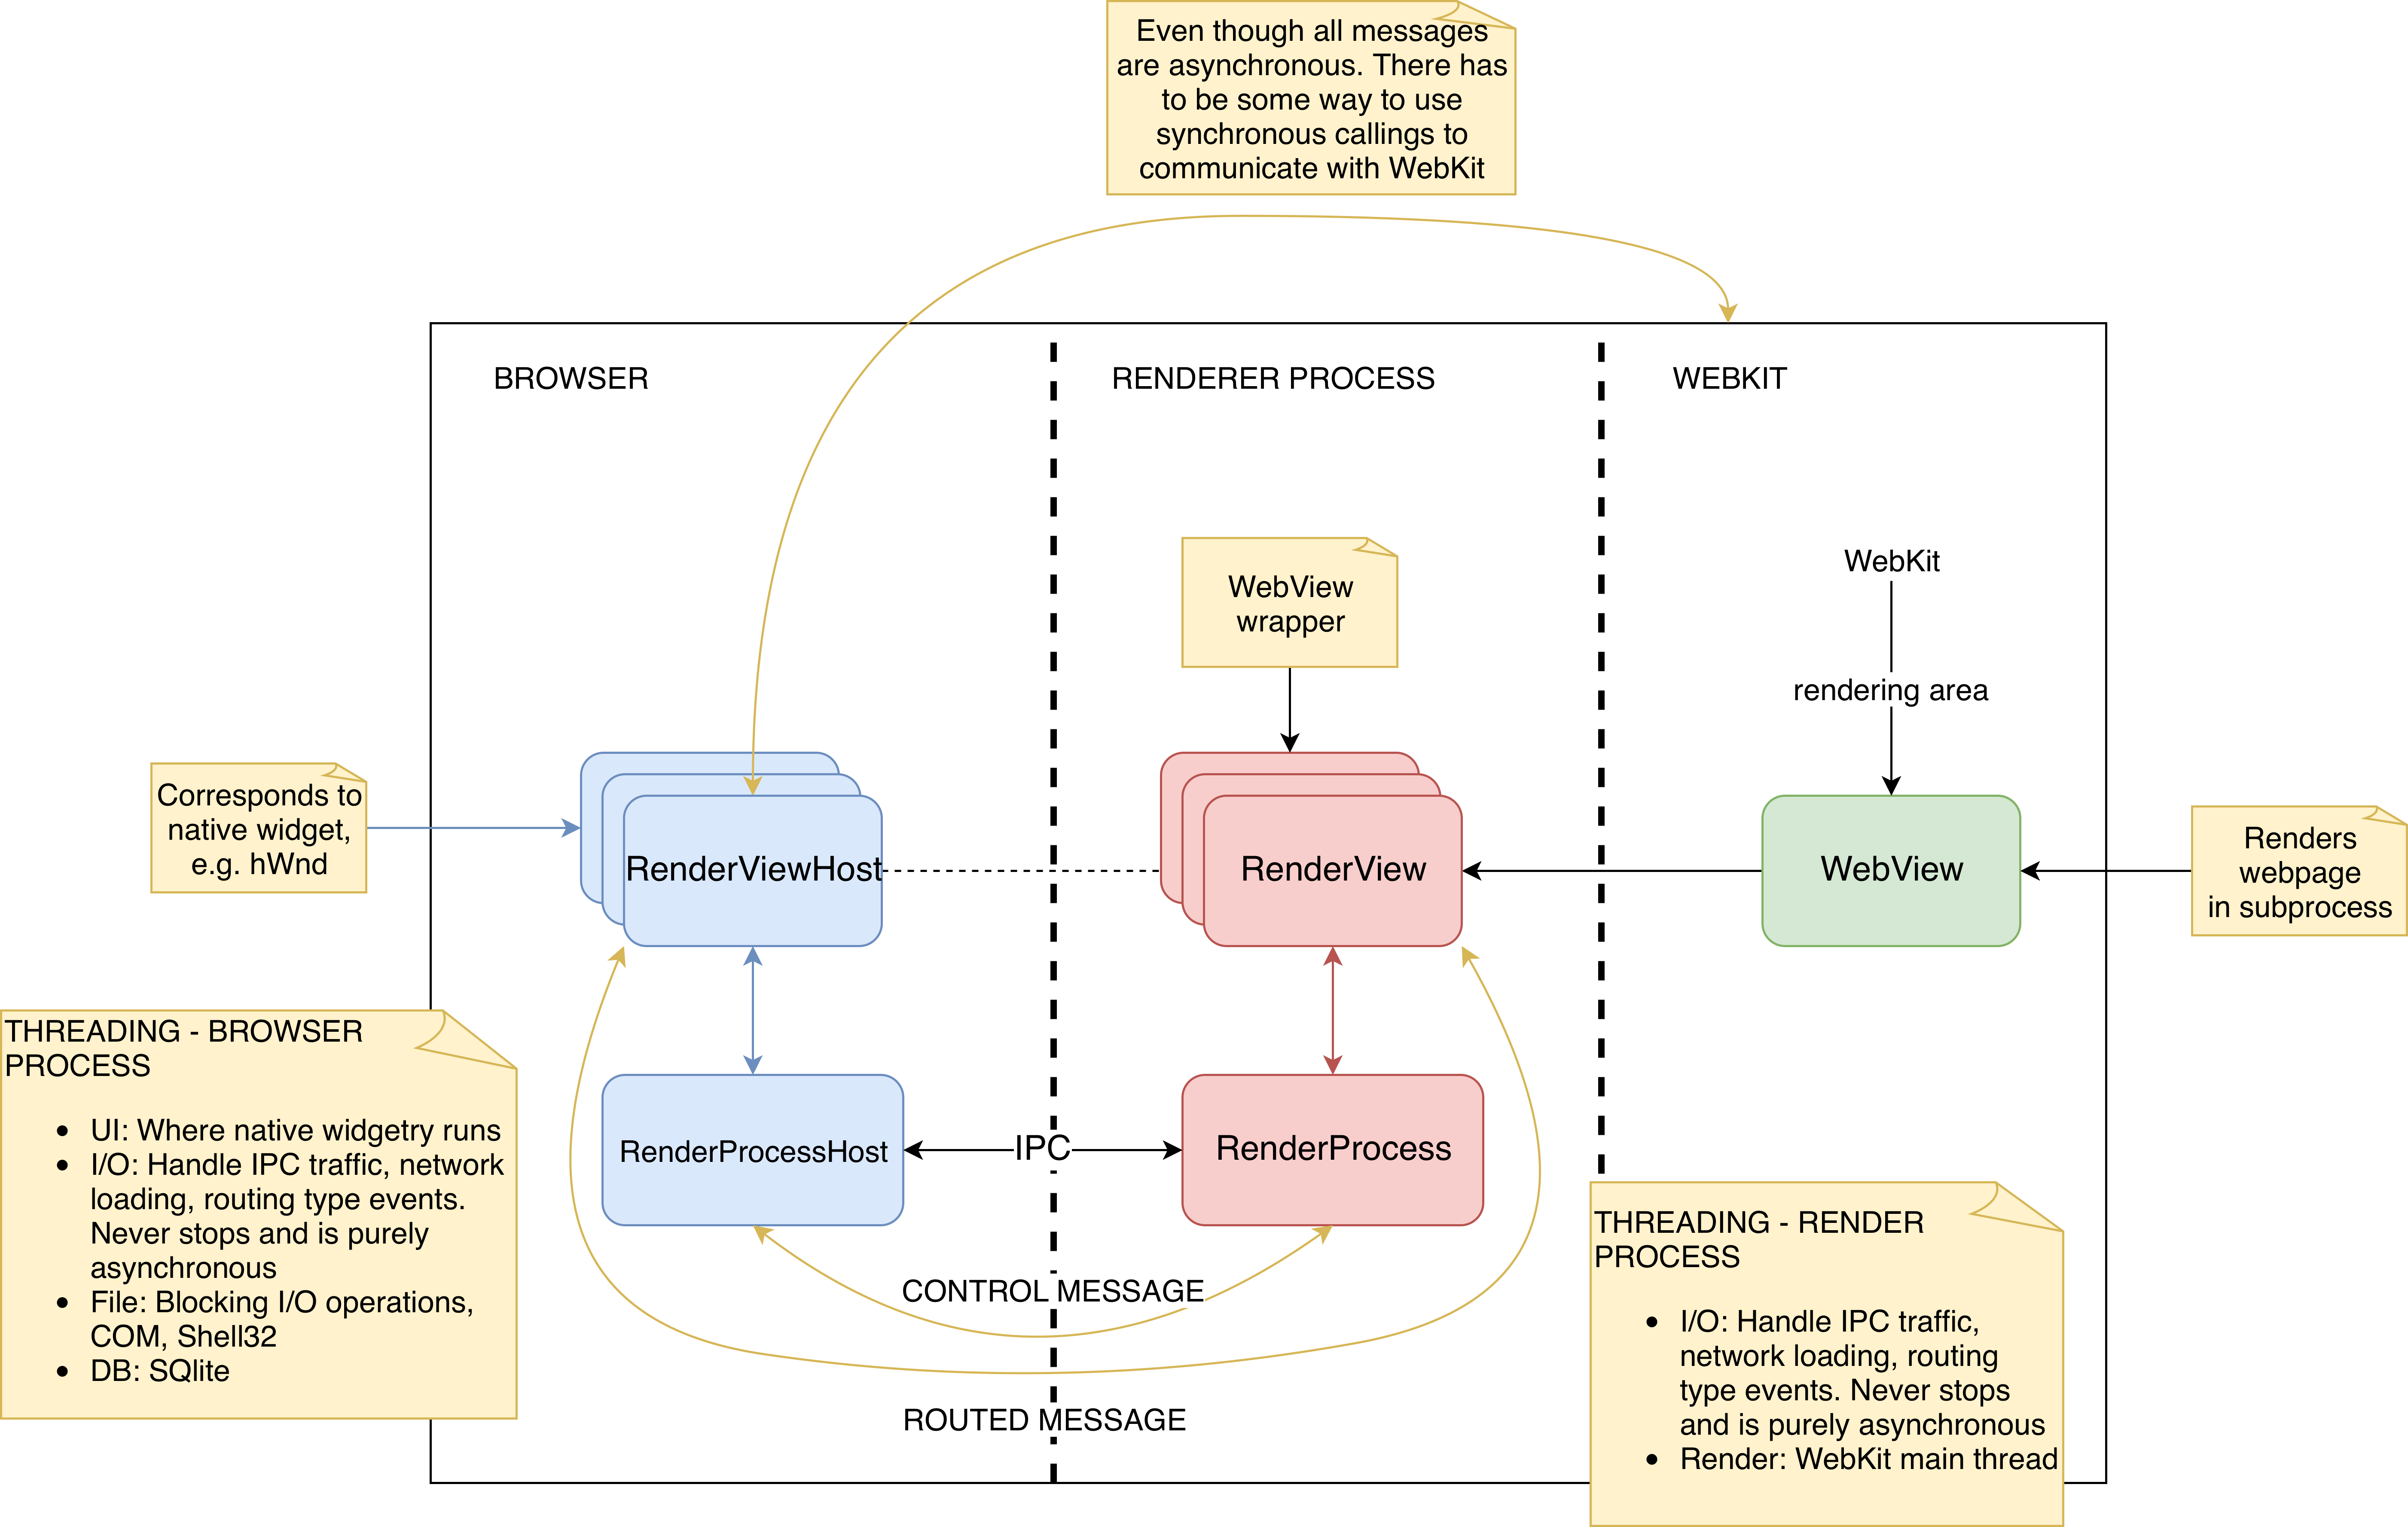
\includegraphics[width=\textwidth]{img/multiprocess.png}
    \caption{Chromium's multi process architecture}
    \label{fig:arch}
\end{sidewaysfigure}

Each render process has one or more \texttt{RenderView} objects, managed by the \texttt{RenderProcess}, which correspond to tabs of content. The corresponding \textit{RenderProcessHost} maintains a \texttt{RenderViewHost} corresponding to each view in the renderer. Each view is given a view ID that is used to differentiate multiple views in the same renderer. These IDs are unique inside one renderer but not within the browser, so identifying a view requires a \texttt{RenderProcessHost} and a view ID. Communication from the browser to a specific tab of content is done through these \texttt{RenderViewHost} objects, which know how to send messages through their \texttt{RenderProcessHost} to the \texttt{RenderProcess} and on to the \texttt{RenderView}.

\subsection{Components and interfaces}

In the render process:
\begin{description}
\item[\texttt{RenderProcess}] Handles IPC with the corresponding \texttt{RenderProcessHost} in the browser. There is exactly one \texttt{RenderProcess} object per render process. This is how all browser renderer communication happens.
\item[\texttt{RenderView}] Communicates with its corresponding \texttt{RenderViewHost} in the browser process (via the \texttt{RenderProcess}), and WebKit embedding layer. This object represents the contents of one web page in a tab or popup window.
\end{description}

\noindent In the browser process:
\begin{description}
\item[\texttt{Browser}] Represents a top-level browser window.
\item[\texttt{RenderProcessHost}] Represents the browser side of a single browser renderer IPC connection. There is one \texttt{RenderProcessHost} in the browser process for each render process.
\item[\texttt{RenderViewHost}] Encapsulates communication with the remote \texttt{RenderView}, and \texttt{RenderWidgetHost} handles the input and painting for \texttt{RenderWidget} in the browser.
\end{description}

\subsection{Process Models}

By default, the browser will spawn a new process and instruct it to create a single \texttt{RenderView}. On the other hand, the architecture also supports assigning new tabs to existing processes due to diverse reasons.

\begin{itemize}
    \item The total number of processes is too large
    \item The user already has an open process with that domain
    \item A web application opens a new window that it expects to communicate with synchronously
\end{itemize}

There are many ways that a web browser could be segmented into different OS processes, and choosing the best architecture depends on many factors, including stability, resource usage, and observations from actual usage. Chromium supports four different process models to allow experimentation, with a default model that best fits most users:

\begin{center}
    \addtolength{\leftskip} {-2cm}
    \addtolength{\rightskip}{-2cm}
    \begin{tabular}{m{0.15\textwidth}>{\centering}m{0.3\textwidth}>{\centering}m{0.3\textwidth}m{0.25\textwidth}}
    \hline
     & \textbf{Overview} & \textbf{Strengths} & \hspace*{0.8cm} \textbf{Weaknesses} \\\cline{2-4} 
    \textbf{Process$\times$site-instance} & \begin{center}One renderer process for each instance of a site\end{center} & \begin{center}$\checkmark$ Isolates content from different sites \\ $\checkmark$ Isolates independent tabs showing the same site\end{center} & \begin{center}$\times$ More memory overhead\end{center} \\ \cline{2-4} 
    \begin{center}\textbf{Process$\times$site}\end{center} & \begin{center}Groups all instances of the same site into the same process.\end{center} & \begin{center}$\checkmark$ Less memory overhead \\ $\checkmark$ Isolates content from different sites\end{center} & \begin{center}$\times$ Can result in large renderer processes\end{center} \\ \cline{2-4} 
    \begin{center}\textbf{Process$\times$tab}\end{center} & \begin{center}One renderer process to each unit of related browsing contexts tabs (e.g: a tab and any other tabs that it opens using \textit{Javascript})\end{center} & \begin{center}$\checkmark$ Simple to understand\end{center} & \begin{center}$\times$ Leads to undesirable fate sharing between pages\end{center} \\ \cline{2-4} 
    \begin{center}\textbf{Single process}\end{center} & \begin{center}For the purpose of comparison\end{center} & \begin{center}$\checkmark$ Easy to implement \\ $\checkmark$ Good for developing purposes \end{center} & \begin{center}$\times$ Not safe nor robust\\ $\times$ Any renderer crash will cause the loss of the entire browser process\end{center} \\ \hline
    \end{tabular}
\end{center}

\subsection{Threading and Inter-process Communication}

Within the browser, communication with the renderers is done in a separate I/O thread. Messages to and from the views then have to be proxied over to the main thread using a \texttt{ChannelProxy}. The advantage of this scheme is that resource requests, which are the most common and performance critical messages, can be handled entirely on the I/O thread and not block the user interface. These are done through the use of a \texttt{ChannelProxy::MessageFilter} which is inserted into the channel by the \texttt{RenderProcessHost}. This filter runs in the I/O thread, intercepts resource request messages, and forwards them directly to the resource dispatcher host. 

Each renderer also has a thread that manages communication (in this case, the main thread), with the rendering and most processing happening on another thread (see the diagram in multi-process architecture). Most messages are sent from the browser to the WebKit thread through the main renderer thread and vice-versa. This extra thread helps support synchronous renderer-to-browser messages.

\subsection{Security point of view}

Chromium's mechanism \cite{sec} for separating running renderers, mitigates system failures or vulnerabilities from spreading, thus, helping protect against malware. For example, it can ensure that the renderer's only access to the network is via its parent browser process. Likewise, it can restrict its access to the filesystem using the host operating system's built-in permissions.

In addition to restricting the renderer's access to the filesystem and network, it can also place limitations on its access to the user's display and related objects, which prevents a compromised renderer from opening new windows or capturing keystrokes. 


\section{Plugin architecture} 
\label{sec:plugin}

Plugins are a major source of browser instability. Plugins also make sandboxing impractical, as plugins are written by third-parties and we can't control their access to the operating system. The solution is to run plugins in their own separate process. Chromium has the ability to run plugins both in process, which is handy for testing, as well as out of process. 
\subsection{In process plugins}
\begin{figure}[H]
    \centering
    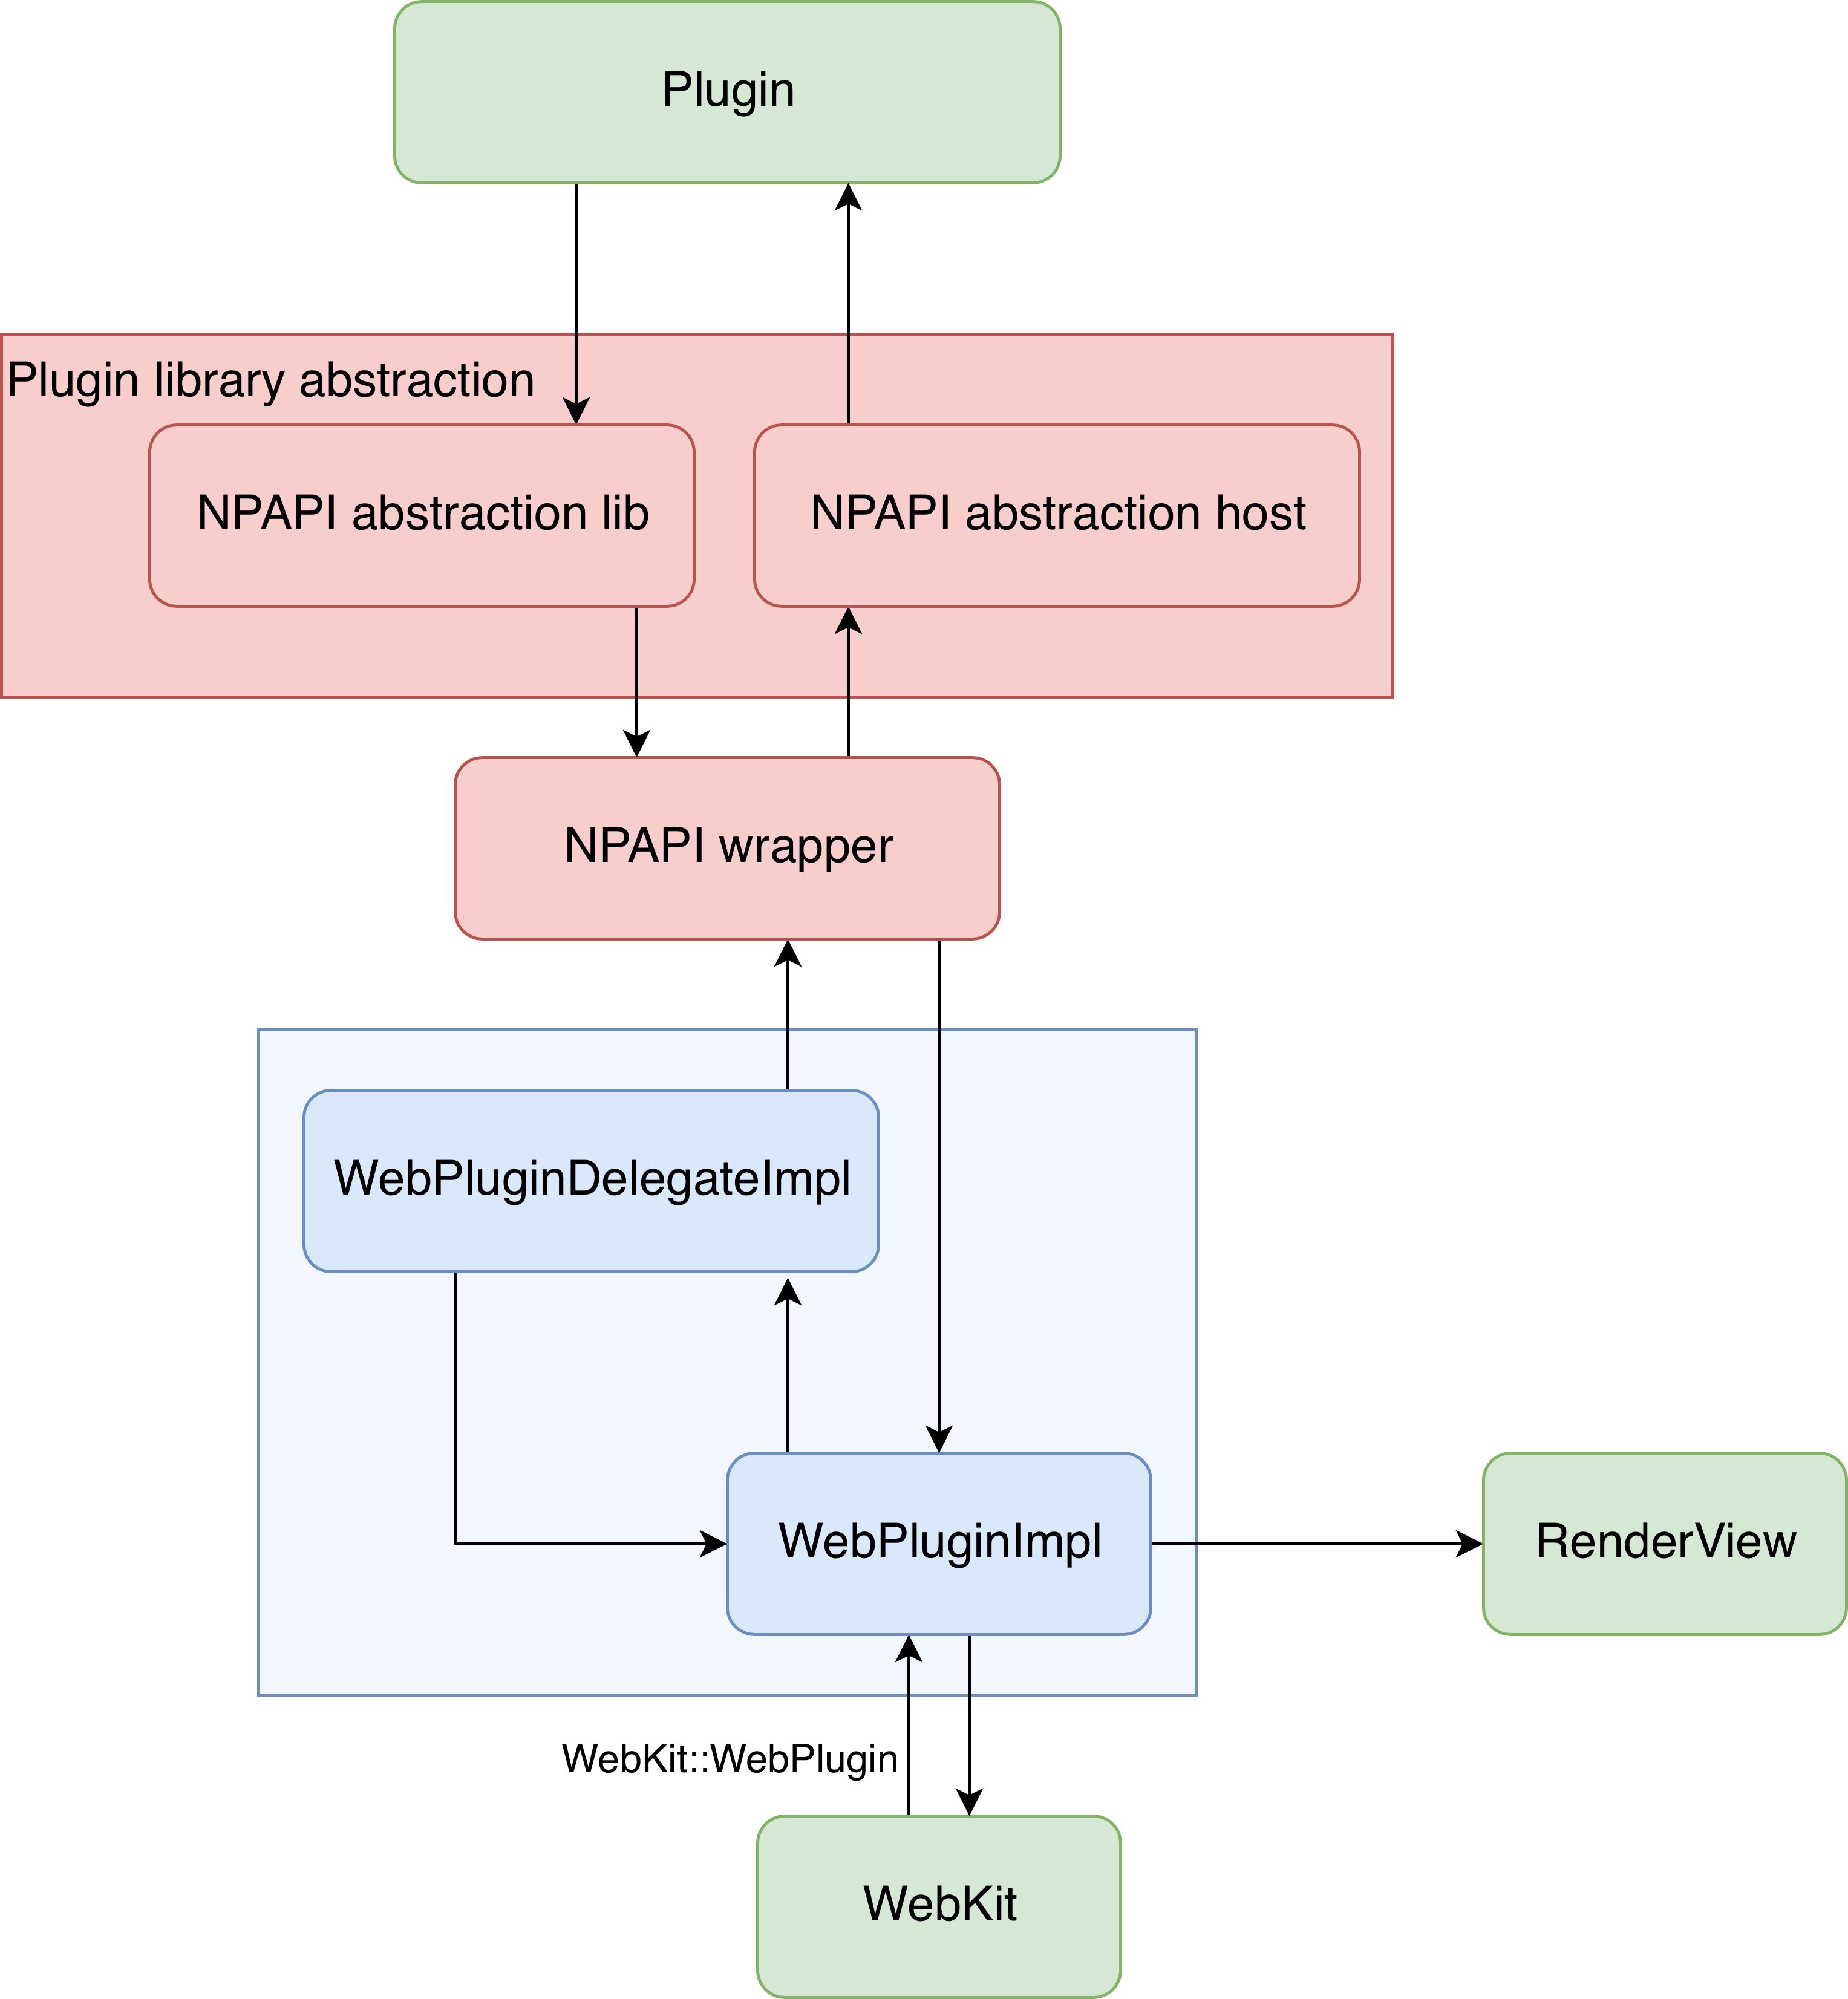
\includegraphics[width=0.8\textwidth]{img/in.png}
    \caption{In process plugin}
    \label{fig:in}
\end{figure}

WebKit embedding layer expects the embedder to implement the \texttt{WebKit::WebPlugin} interface. This is implemented by \texttt{WebPluginImpl}. The WebPluginImpl talks ``up" the chain to a \texttt{WebPluginDelegate} interface. This in turn talks to our NPAPI wrapper layer. Figure \ref{fig:in} represent the aforementioned description.

\subsection{Out of process plugins}

The layer indicated by the dotted line in figure \ref{fig:out} interposes an IPC cover between the \texttt{WebPluginImpl} and \texttt{WebPluginDelegateImpl} layers seen in figure \ref{fig:in}. The two sides of the \texttt{Renderer/Plugin} communication channel are represented by the \texttt{Channel} and the \texttt{ChannelHost} components. Since each unique plugin may be present in many renderer processes, this means there must be one \texttt{ChannelHost} for each type of plugin it uses. Similarly, every plugin process has a Channel component for each renderer process.

\begin{figure}[H]
    \centering
    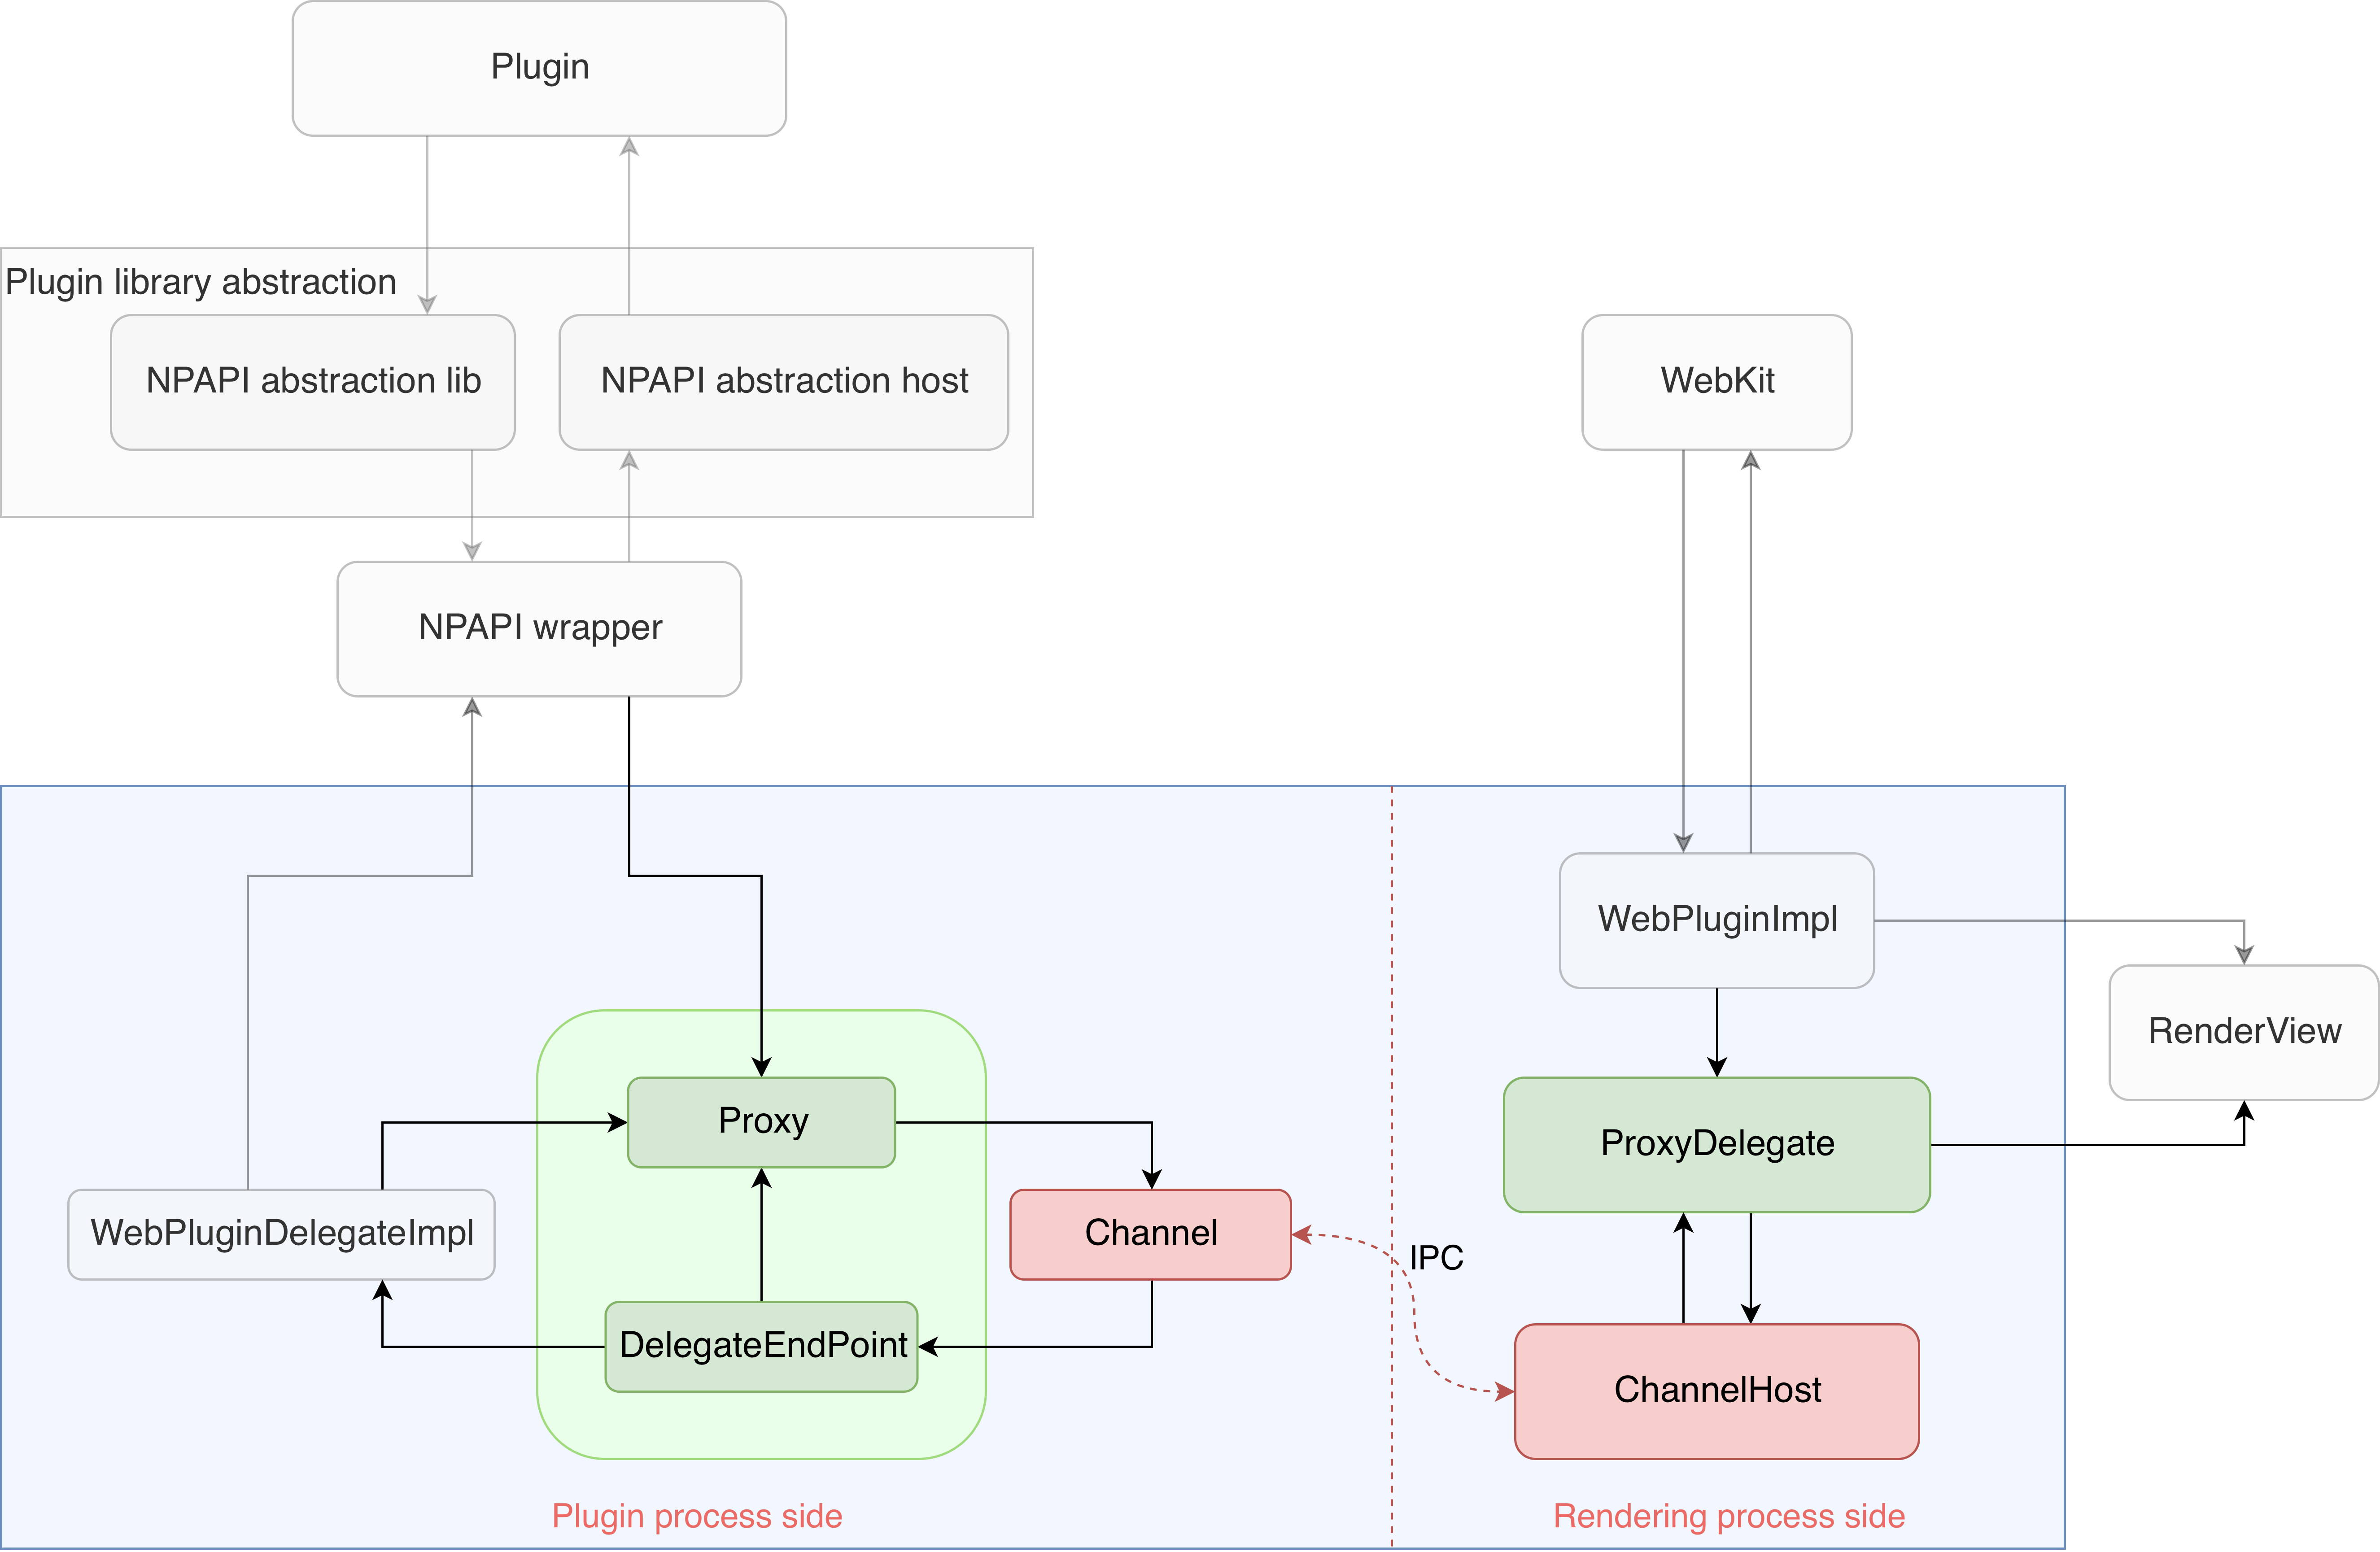
\includegraphics[width=\textwidth]{img/chromium-out.png}
    \caption{Out of process plugin}
    \label{fig:out}
\end{figure}

Each end of the channel, in turn, maps to many different instances of a plugin. The channel is in charge of multiplexing the communication between these many objects over one IPC connection.


\section{Alternative architecture}

From the standpoint of the aforementioned concepts, where we summarize the multi-process architecture's main advantages, we found that there is no other architecture that could replace this one maintaining its core functionalities, that synergize so well with the project philosophy.

Therefore, and under our humble point of view, this architecture is a perfect counterpart and the main motive as to why the application achieves its purposes and user expectatives.